\section{Probleem Analyse en Eisen}

In deze sectie worden de beperkingen van de huidige testopstelling opgesomt en waarom deze beperkingen momenteel een probleem vormen.

\subsection{Huidige Situatie}

In de testkast zit de AX5140 servo drive geïnstalleerd (Figuur \ref{fig:AX5140}). Deze drive is uitgebreidt met een AX5801-0200 veiligheidskaart waardoor het mogelijk is om veiligheids functies zoals Safe Torque Off (\gls{STO}) te configureren om veilig (en snel) tot stilstand te komen.

\vspace{0.5cm}

De AX5140 servo drive ondersteunt standaard niet alle encoder protocollen en is daarom uit uitgebreid met de AX5701 Encoder optie kaart zodat bijvoorbeeld EnDat en Hiperface encoders ook aangesloten kunnen worden.

\vspace{0.5cm}

Het testprogramma die momenteel op de testkast staat bevat maar één parameter set voor één type motor. Zelfs wanneer er meer parameter sets aanwezig zouden zijn is er in het huidige programma geen manier om deze automatisch te schrijven naar de drive heen. Nieuwe parametersets zullen handmatig met TwinCAT XAE naar de drive moeten worden geschreven. Dit kan tijdsintensief zijn en lastig zijn voor mensen die dit nooit eerder gedaan hebben het is daarom wenselijk om dit zo makkelijk mogelijk te maken.

\begin{figure}[h]
	\centering
	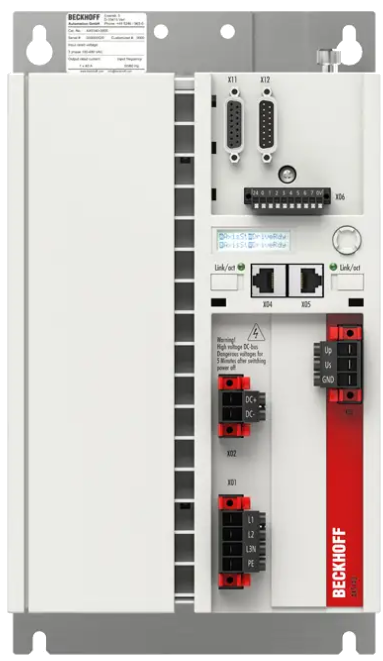
\includegraphics[width=150pt]{AX5140}
	\label{fig:AX5140}
	\caption{De \gls{AX5140} motordrive \cite{web:AX5140Drive}}
\end{figure}

\newpage

\subsection{Eisen}

Hieronder staan de belangrijkste eisen van de testopstelling van dit onderzoek. Voor alle eisen wordt doorverwezen naar het SRD bestand van de testopstelling (bijlage \ref{sec:TestKastSRD}).

